

% DISTRIBUTION %%%%%%%%%%%%%%%%%%%%%%%%%%%%%%%%%%%%%%%%%%%%%%%%
\section{Spatial distribution of forest and seed attributes} \label{app:spatial_distri}

% Across all plots in both dry and wet tropical forest 116 unique species were collected during the one-year sampling period. In the wet forest, species richness was higher with 71 unique species and on average 14.25 species per plot, while in the dry forest 45 unique species were identified with on average 7.25 species per plot. 

% In the dry tropical forest 83\% of seeds were abiotically dispersed whereas in the wet tropical forest 63.7\% of seeds were abiotically dispersed. The biotic dispersal is, however, notably higher for the wet tropical forest (27.2\%) compared to the dry tropical forest (3.5\%). The remainder of the seeds were either dispersed by both, biotic and abiotic dispersal mode, or the dispersal mode was unknown.

% The composition of the guild groups also  followed a similar pattern between the forest types. Pioneer species dominated the seed rain in both dry (48.5\%) and wet (57.4\%) tropical forest, followed by the generalist species representing 15.6\% of species in the dry forest type 21.7\% of species in the wet forest type. The least represented group was the shade-tolerant species with 8.6\% of species in the dry forest and 9.3\% of species in the wet forest. The remained of the seeds had their dispersal mode unknown.

% For visual interpretation, Fig. \ref{fig:distribution_dry} and Fig. \ref{fig:distribution_wet} represent the spatial distribution of richness, dispersal modes and guild types in both dry and wet tropical forest per research plot. Lastly, Fig. \ref{fig:boxplot res} illustrates  boxplot distribution of each seed variable between dry and wet tropical forest. 

% The surrounding landscape varied between the two forest types. In dry tropical forest, on average research plots were surrounded 74.6\% of forest, whereas in wet tropical forest, the research plots were surrounded by only 37.5\% of forest on average.

% Forest successional stage composition differed between the two regions. The dry forest type was dominated by late successional forest representing on average 88.5\% of the forest cover  with the reminder belonging to the early successional forest. In the wet forest, the forest cover surrounding the research plot was almost equally divided between the two groups with 56.5\% belonging to the late successional forest and reminder belonging to the early successional forest. 

% Patterns of forest connectivity also contrasted between forest types. On average, plots in the dry forest were embedded in more connected forest landscapes (0.0153) compared to those in the wet forest (0.0126). This corresponds with the high percentage of forest cover in the dry vs wet forest type.

% For visual interpretation, Fig. \ref{fig:radius_dry} and Fig. \ref{fig:radius_wet} represent the surrounding landscape around each research plot. Lastly, Fig. \ref{fig:boxplot_pred} illustrates  boxplot distribution of each forest variable between dry and wet tropical forest. 



% First figure
\begin{figure}[H]
\centering
\setlength{\fboxrule}{12pt}
\setlength{\fboxsep}{0pt}
\fcolorbox{framecol}{white}{%
  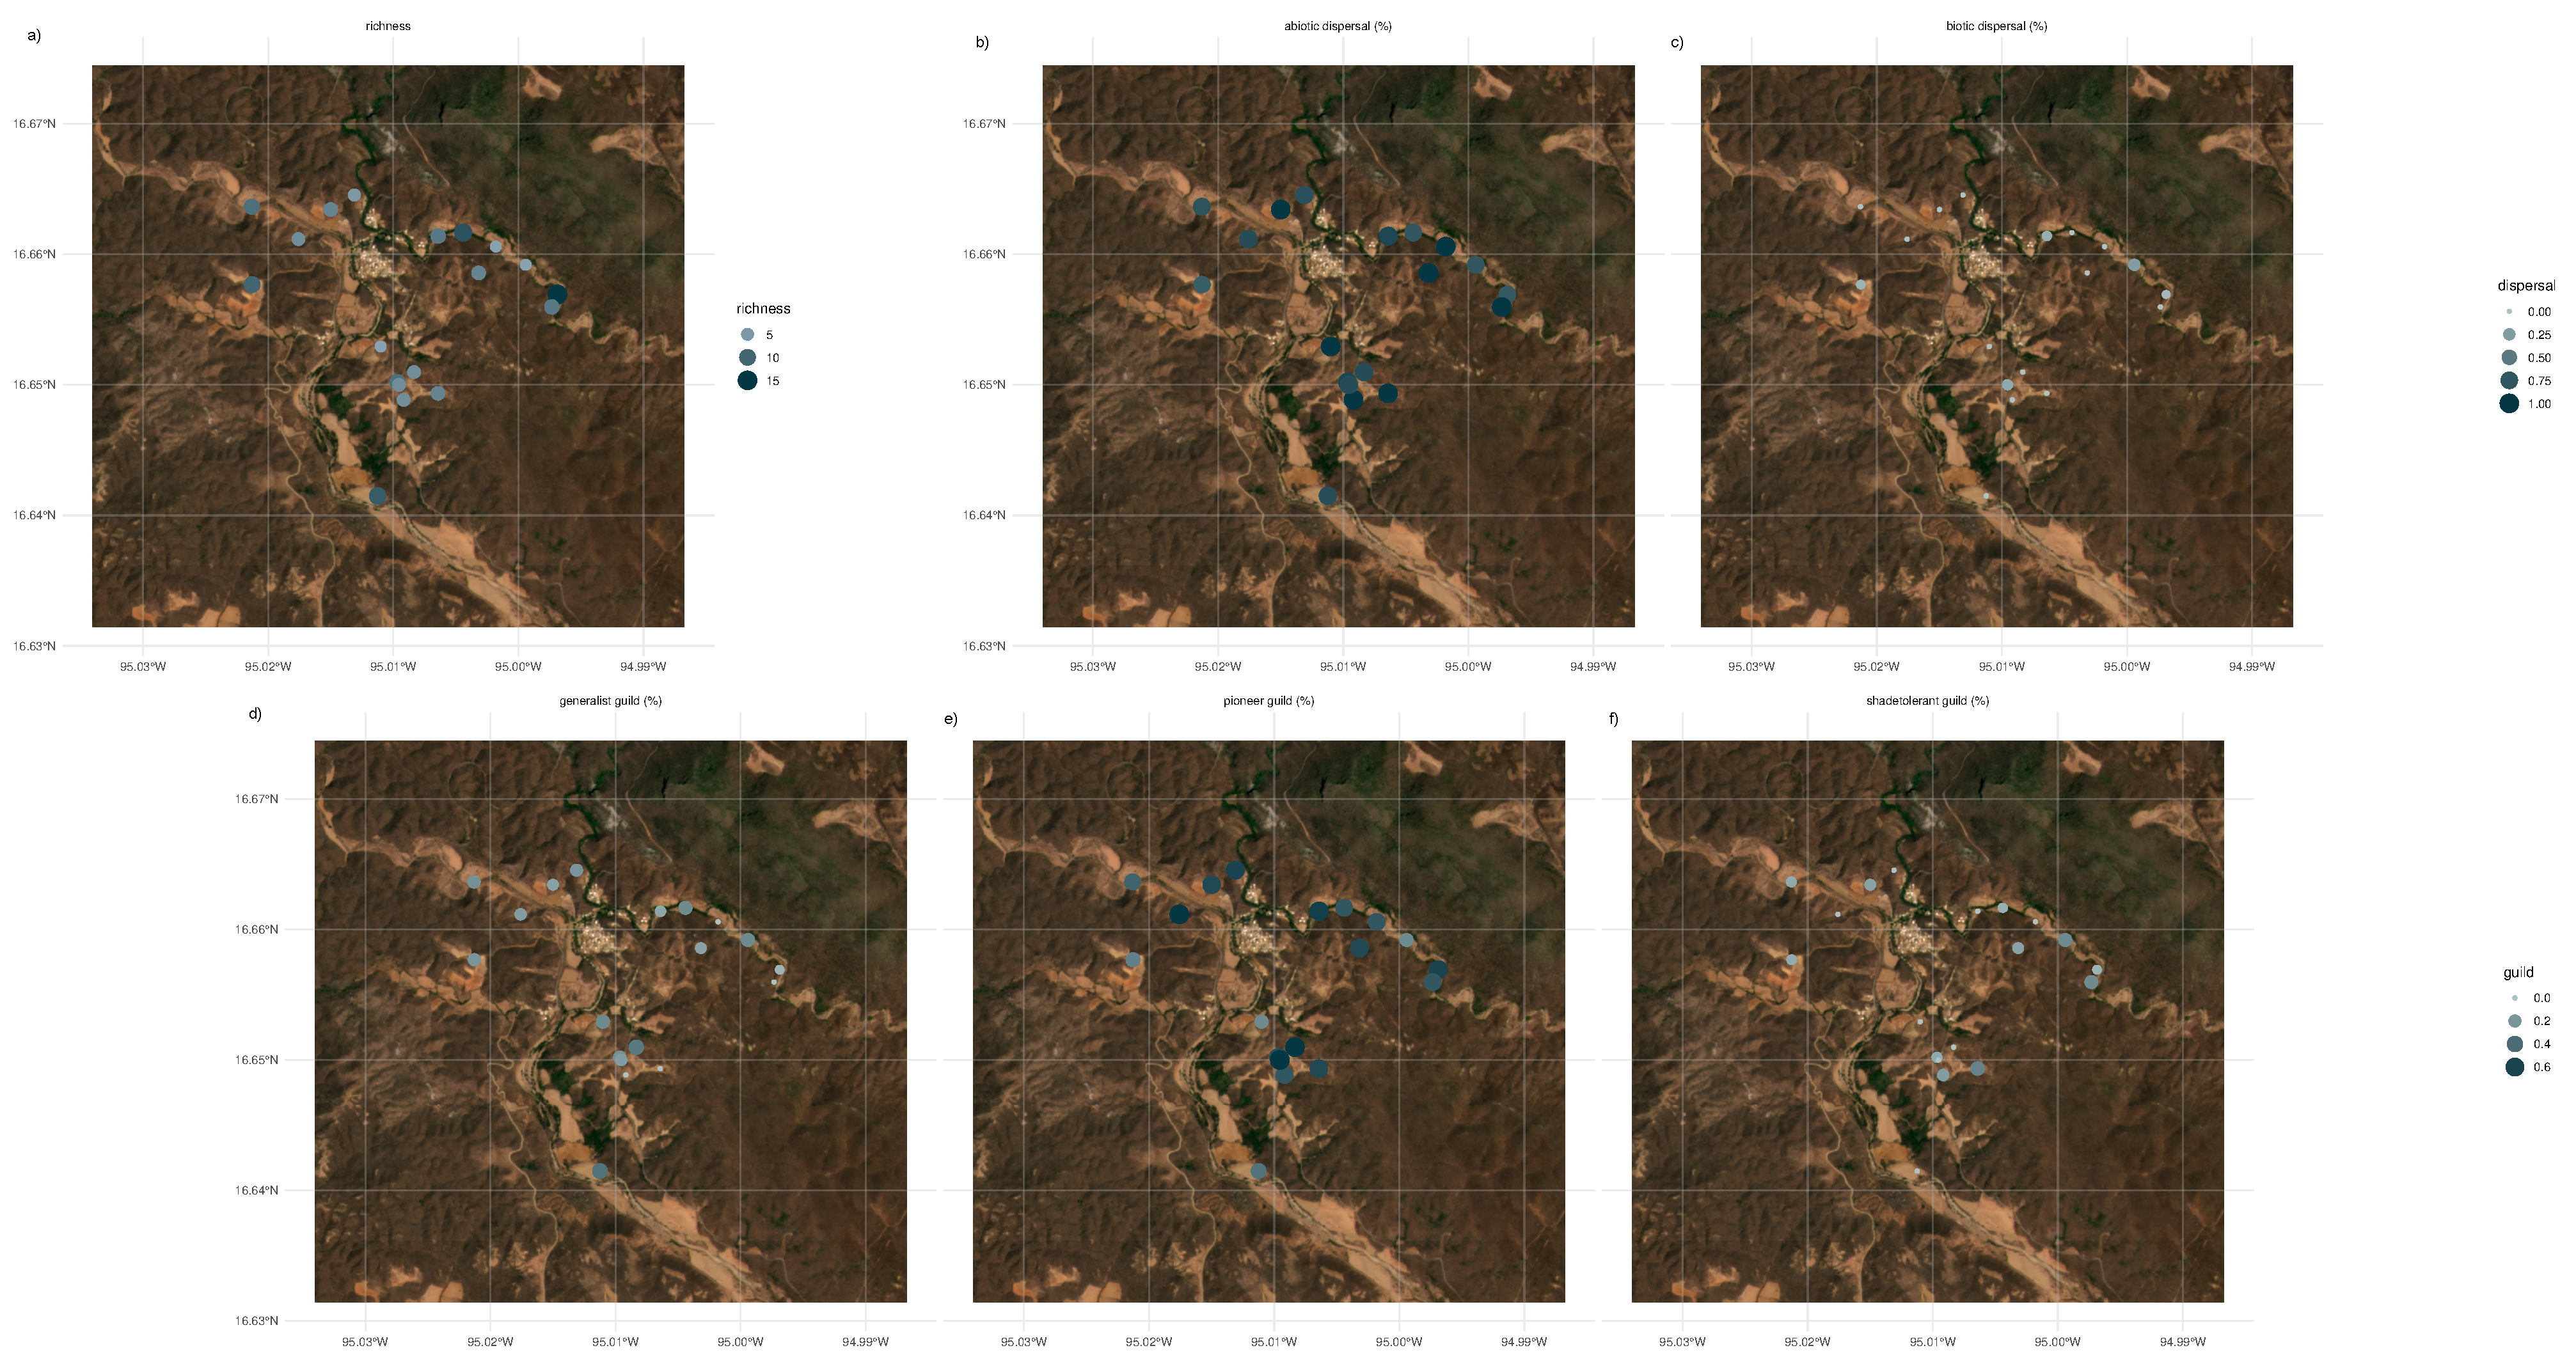
\includegraphics[width=\linewidth, keepaspectratio]{Report/figures/a1_distribution_dry.pdf}%
}
\caption{\textit{Spatial distribution of seed attributes across regenerating forest research plots in the dry tropical forest of Oaxaca, Mexico. Circle size represents the magnitude of each variable at a given plot. Images represent a) seed species richness, b) proportion of abiotically dispersed seeds, c) proportion of biotically dispersed seeds, d) proportion of generalist, e) pioneer and f) shade-tolerant guilds. The background map shows the satellite imagery of the landscape derived from Planet 2021 (q3) \citep{planet}. Research plots were overlaid according to their geographic coordinates.}}
\label{fig:distribution_dry}
\end{figure}

% Second figure
\begin{figure}[H]
\centering
\setlength{\fboxrule}{12pt}
\setlength{\fboxsep}{0pt}
\fcolorbox{framecol}{white}{%
  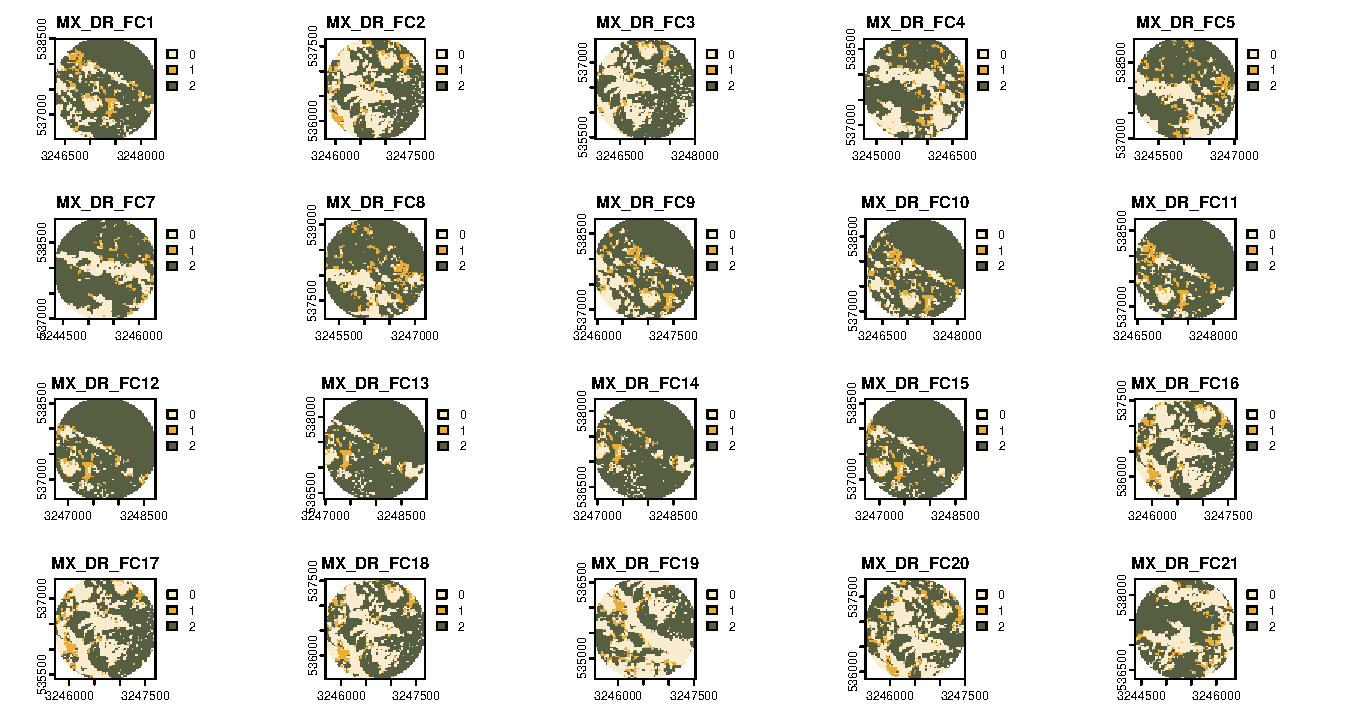
\includegraphics[width=\linewidth, keepaspectratio]{Report/figures/a2_extractedradius_dry.pdf}%
}
\caption{\textit{Maps showing the surrounding landscape context of 20 regenerating forest research plots located in the dry tropical forest of Oaxaca, Mexico. Each panel (MX\_DR\_FC1–FC21, MX: Mexico, DR: dry, FCn: number of research plot) shows a circular landscape window (r = 1000~m) centered on a plot, with land cover classified into three categories: 0 = non-forest , 1 = early successional forest ($\le$ 30 years), and 2 = late successional forest ($>$ 30 years).}}
\label{fig:radius_dry}
\end{figure}



% First figure
\begin{figure}[H]
\centering
\setlength{\fboxrule}{12pt}
\setlength{\fboxsep}{0pt}
\fcolorbox{framecol}{white}{%
  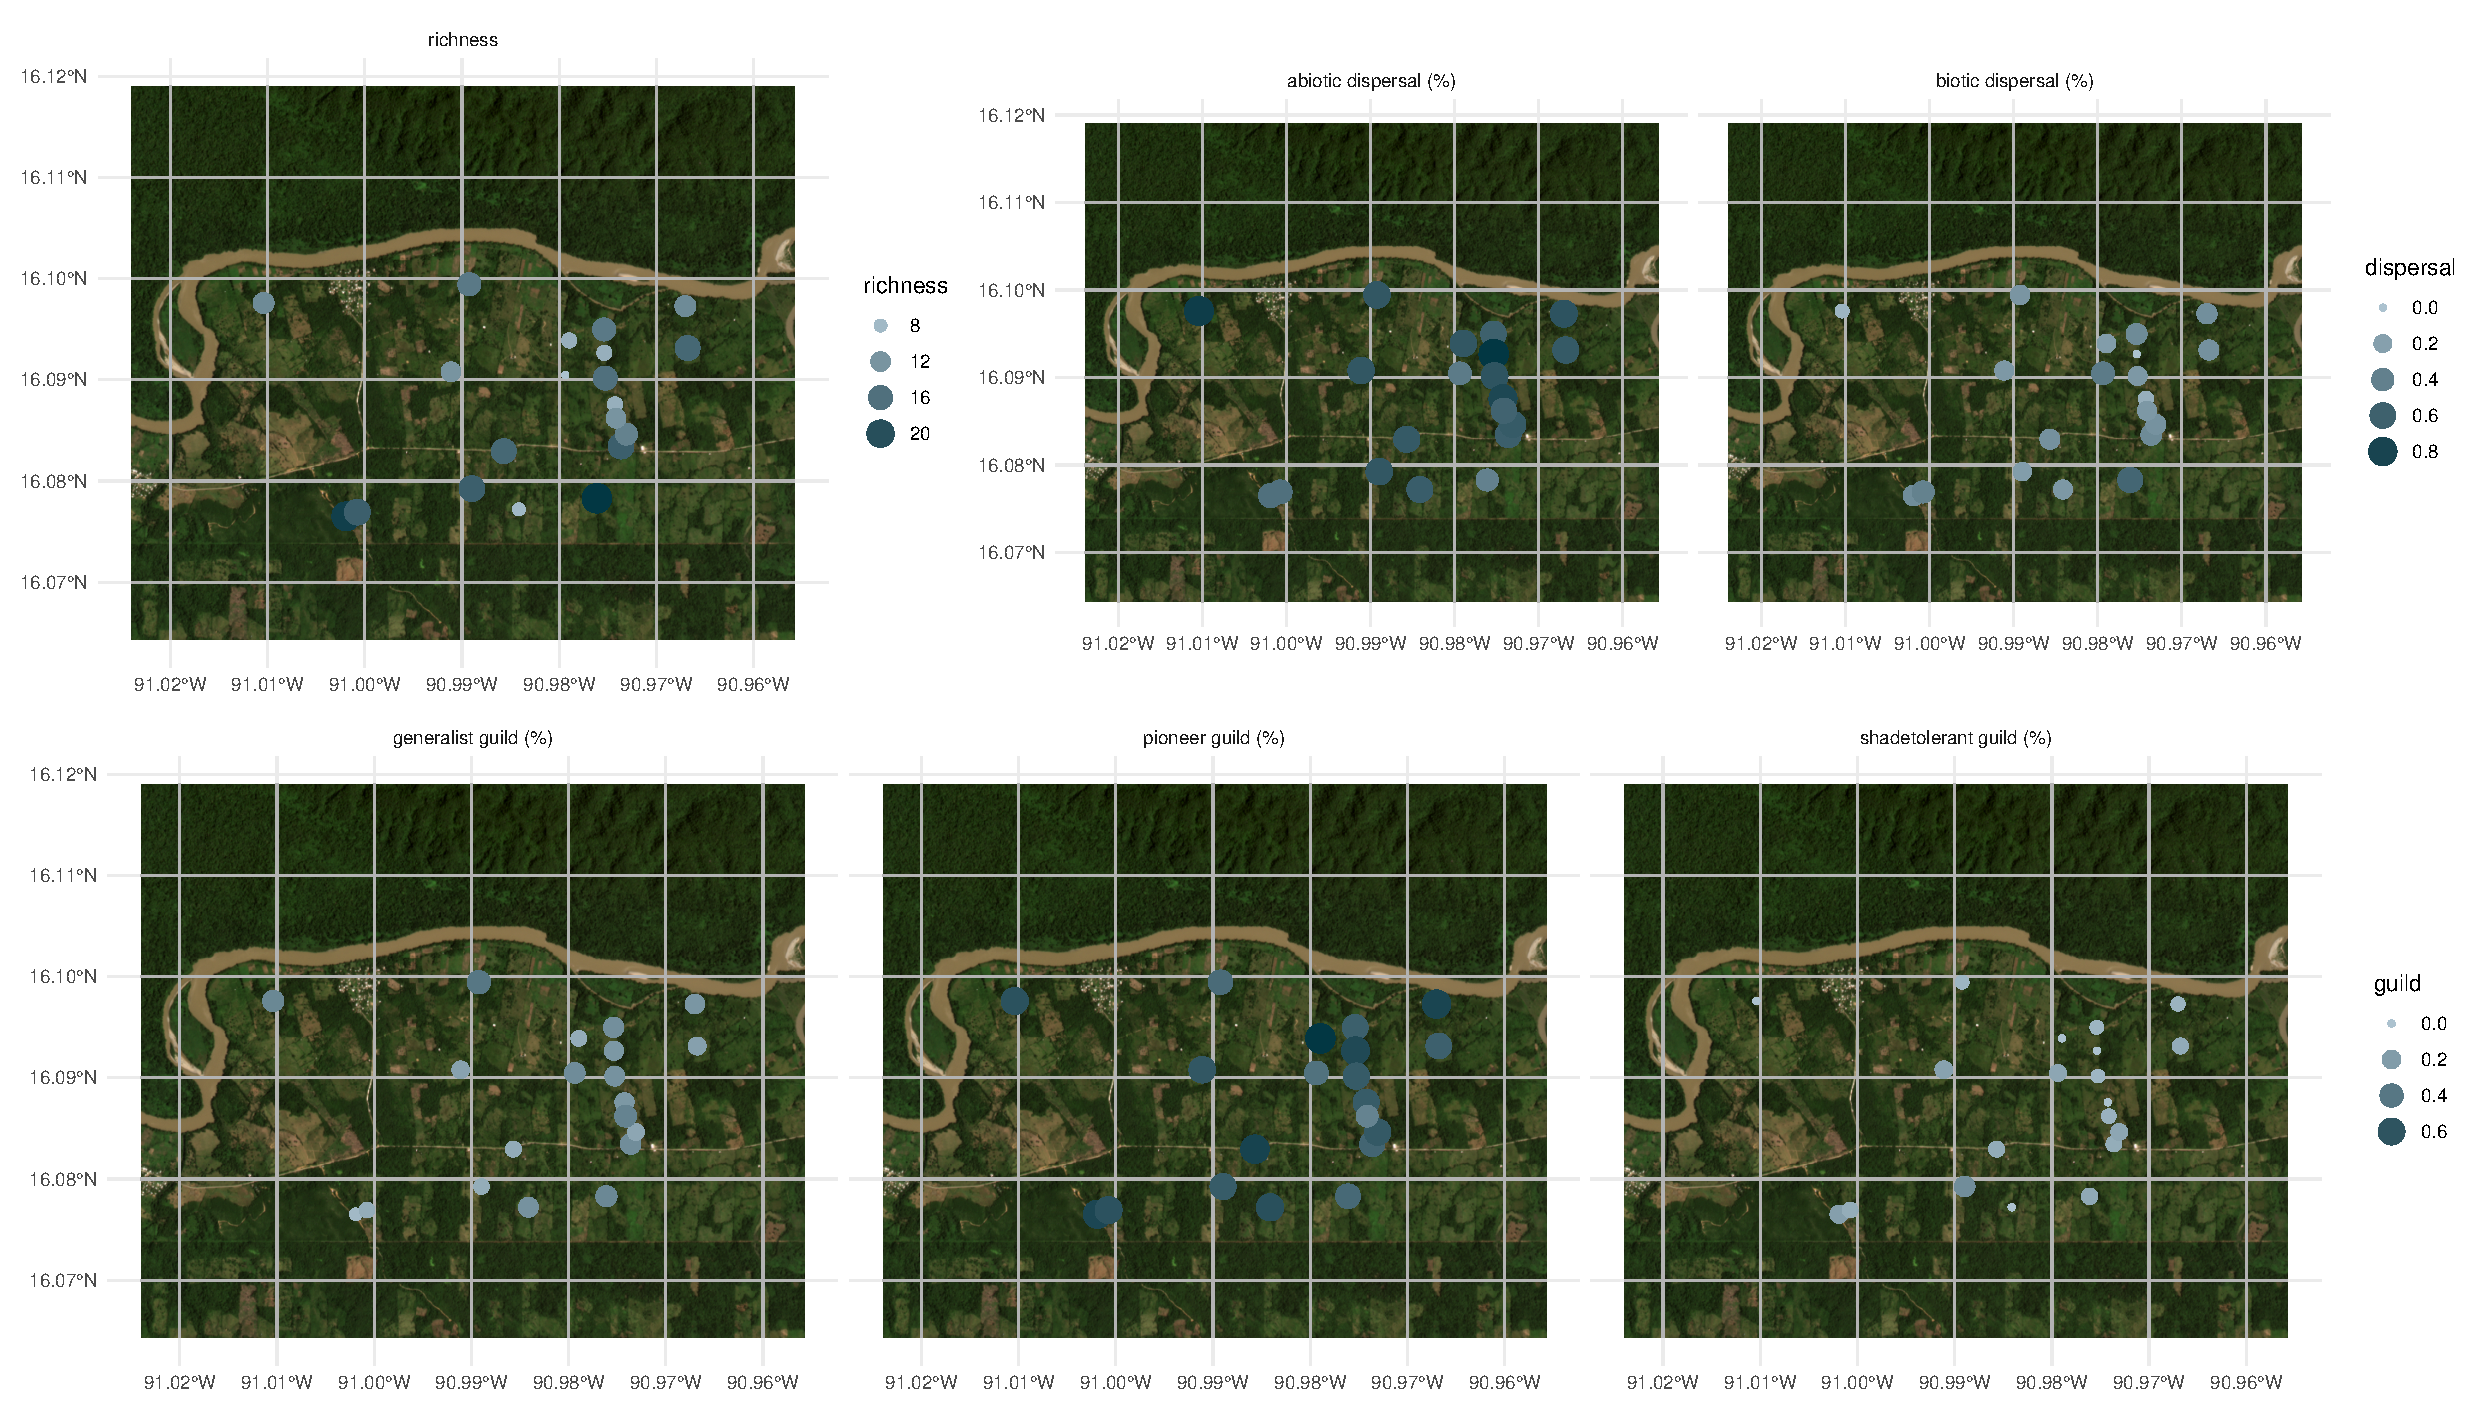
\includegraphics[width=\linewidth, keepaspectratio]{Report/figures/a3_distribution_wet.pdf}%
}
\caption{\textit{Spatial distribution of seed attributes across regenerating forest research plots in the wet tropical forest of Chiapas, Mexico. Circle size represents the magnitude of each variable at a given plot. Images represent a) seed species richness, b) proportion of abiotically dispersed seeds, c) proportion of biotically dispersed seeds, d) proportion of generalist, e) pioneer and f) shade-tolerant guilds. The background map shows the satellite imagery of the landscape derived from Planet 2021 (q1) \citep{planet}. Research plots were overlaid according to their geographic coordinates.}}
\label{fig:distribution_wet}
\end{figure}

% Second figure
\begin{figure}[H]
\centering
\setlength{\fboxrule}{12pt}
\setlength{\fboxsep}{0pt}
\fcolorbox{framecol}{white}{%
  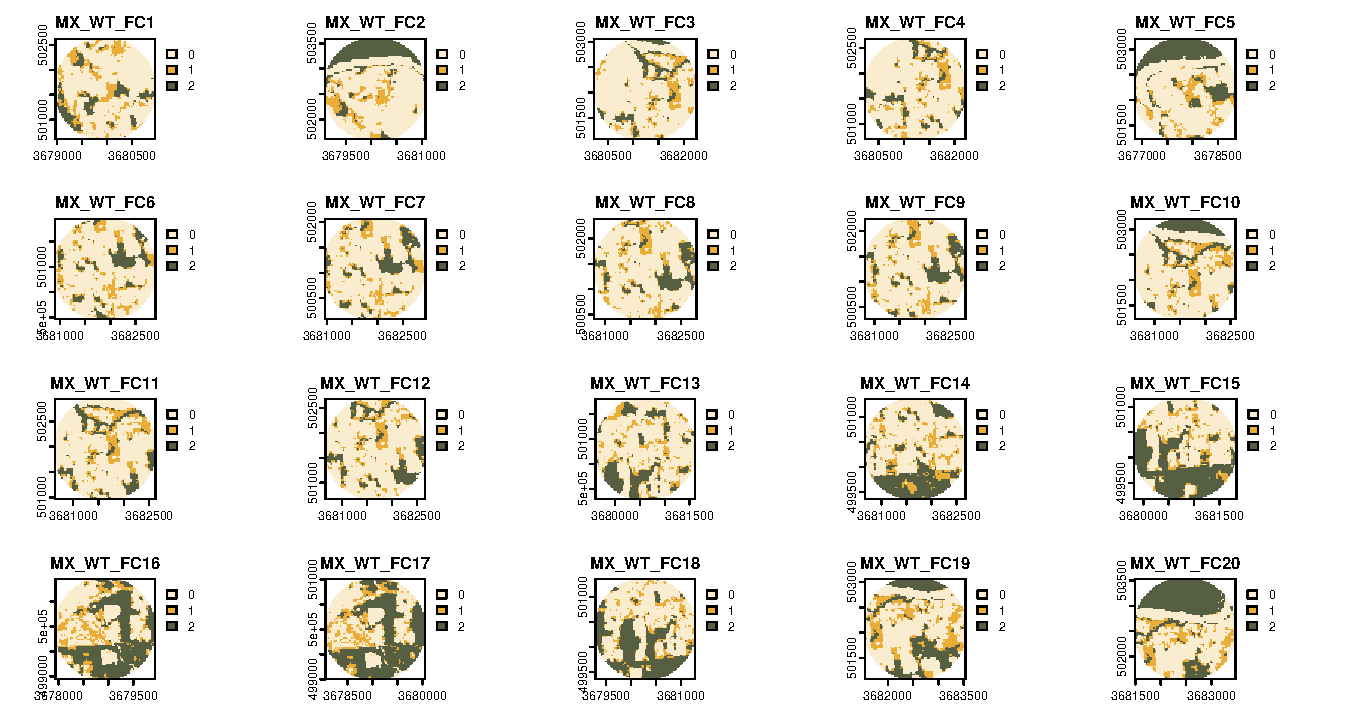
\includegraphics[width=\linewidth, keepaspectratio]{Report/figures/a4_extractedradius_wet.pdf}%
}
\caption{\textit{Maps showing the surrounding landscape context of 20 regenerating forest research plots located in the wet tropical forest of Chiapas, Mexico. Each panel (MX\_DR\_FC1–FC21, MX: Mexico, DR: dry, FCn: number of research plot) shows a circular landscape window (r = 1000~m) centered on a plot, with land cover classified into three categories: 0 = non-forest, 1 = early successional forest ($\le$ 30 years), and 2 = late successional forest ($>$ 30 years).}}
\label{fig:radius_wet}
\end{figure}




\newpage
% MODELS %%%%%%%%%%%%%%%%%%%%%%%%%%%%%%%%%%%%%%%%%%%%%%%%%%
\section{Model results}\label{app:mod_res}

% richness ---------------------------------------------------
\begin{table}[H]
\centering
\scriptsize % smaller font
\caption{\textit{Linear regression results for the relationship between seed species richness and forest attributes. Models (1)–(3) test the effects of forest cover, successional stage, connectivity, and forest type (wet vs. dry) on woody perennial seed richness. Standard errors are in parentheses.}}
\begin{tabularx}{\textwidth}{@{\extracolsep{3pt}}lXXX} 
\\[-1ex]\hline 
\hline \\[-1ex] 
 & \multicolumn{3}{c}{\textit{Dependent variable: Richness}} \\ 
\\[-1ex] & (1) & (2) & (3)\\ 
\hline \\[-0.8ex] 
Forest cover & 1.806 &  &  \\ 
 & (1.272) &  &  \\ 
Forest early successional stage &  & $-$2.652$^{*}$ &  \\ 
 &  & (1.390) &  \\ 
Forest late successional stage &  &  & 2.652$^{*}$ \\ 
 &  &  & (1.390) \\ 
Forest connectivity & $-$0.263 & $-$0.380 & $-$0.380 \\ 
 & (1.064) & (1.030) & (1.030) \\ 
Forest type (wet) & 9.624$^{***}$ & 11.044$^{***}$ & 11.044$^{***}$ \\ 
 & (2.474) & (2.677) & (2.677) \\ 
Constant & 5.938$^{***}$ & 5.228$^{***}$ & 5.228$^{***}$ \\ 
 & (1.382) & (1.468) & (1.468) \\ 
\hline \\[-0.8ex] 
Observations & 40 & 40 & 40 \\ 
R$^{2}$ & 0.488 & 0.509 & 0.509 \\ 
Adjusted R$^{2}$ & 0.445 & 0.468 & 0.468 \\ 
Residual Std. Error (df = 36) & 3.900 & 3.819 & 3.819 \\ 
F Statistic (df = 3; 36) & 11.443$^{***}$ & 12.447$^{***}$ & 12.447$^{***}$ \\ 
\hline 
\textit{Note:} & \multicolumn{3}{r}{$^{*}$p$<$0.1; $^{**}$p$<$0.05; $^{***}$p$<$0.01} \\ 
\end{tabularx} 
\label{tab:richness}
\end{table} 

\vspace{-2ex} % reduce space between table and figure

\begin{figure}[H]
\centering
\scriptsize % smaller caption font
\setlength{\fboxrule}{10pt}  % thinner frame
\setlength{\fboxsep}{0pt}    % no padding
\fcolorbox{framecol}{white}{%
  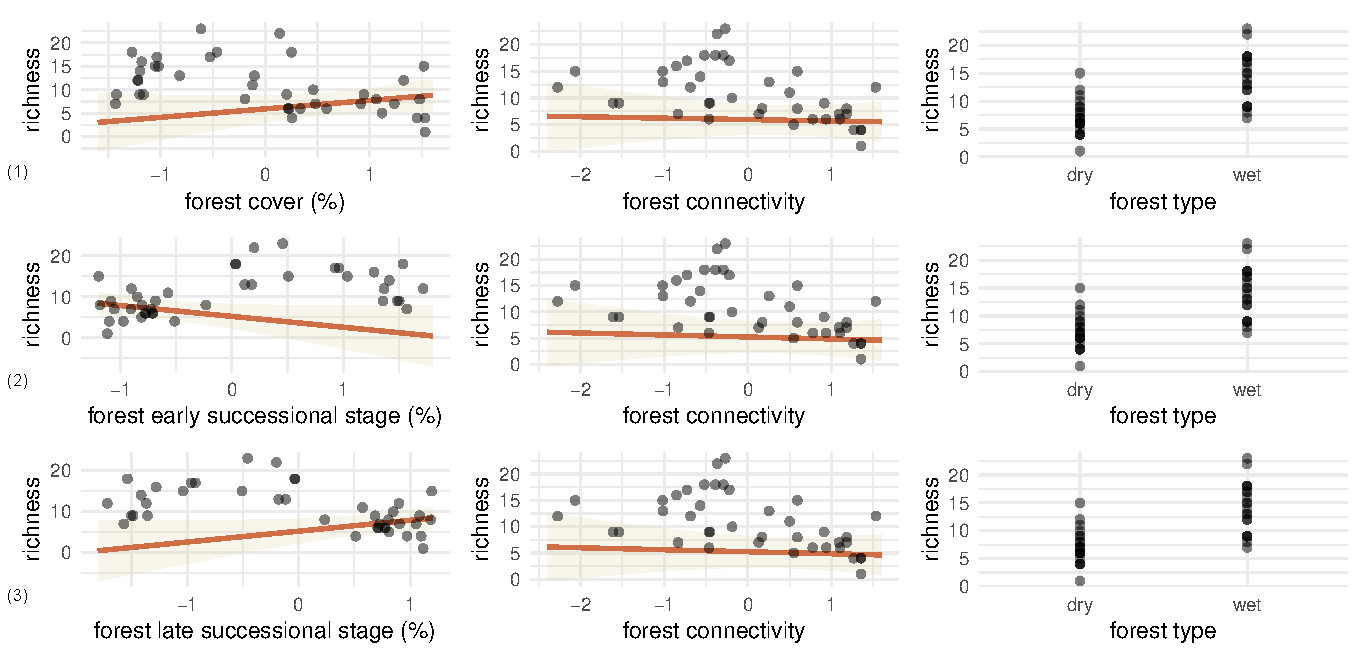
\includegraphics[width=0.95\linewidth,height=0.55\textheight,keepaspectratio]{Report/figures/models_richness.pdf}%
}
\caption{\textit{Relationships between woody perennial seed species richness and forest attributes. Each point represents the annual seed trap measurement per research plot. Linear regression lines (red) with 95\% confidence intervals (orange) show model predictions for models (1)-(3).}}
\label{fig:mod_richness}
\end{figure}


% biotic dispersal -----------------------------------------
\newpage
\begin{table}[H]
\centering
\scriptsize % smaller font
\caption{\textit{Linear regression results for the proportion of biotically dispersed seeds. Models (1)–(3) test the effects of forest cover, successional stage, connectivity, and forest type (wet vs. dry) on the proportion of biotically dispersed seeds of woody perennials. Standard errors are in parentheses.}}
\begin{tabularx}{\textwidth}{@{\extracolsep{3pt}}lXXX} 
\\[-1ex]\hline 
\hline \\[-1ex] 
 & \multicolumn{3}{c}{\textit{Dependent variable: Biotic dispersal}} \\ 
\\[-1ex] & (1) & (2) & (3)\\ 
\hline \\[-0.8ex] 
Forest cover & 0.037 &  &  \\ 
 & (0.053) &  &  \\ 
Forest early successional stage &  & $-$0.030 &  \\ 
 &  & (0.059) &  \\ 
Forest late successional stage &  &  & 0.030 \\ 
 &  &  & (0.059) \\ 
Forest connectivity & 0.039 & 0.043 & 0.043 \\ 
 & (0.044) & (0.044) & (0.044) \\ 
Forest type (wet) & 0.530$^{***}$ & 0.526$^{***}$ & 0.526$^{***}$ \\ 
 & (0.103) & (0.114) & (0.114) \\ 
Constant & 0.031 & 0.033 & 0.033 \\ 
 & (0.057) & (0.062) & (0.062) \\ 
\hline \\[-0.8ex] 
Observations & 40 & 40 & 40 \\ 
R$^{2}$ & 0.646 & 0.643 & 0.643 \\ 
Adjusted R$^{2}$ & 0.616 & 0.613 & 0.613 \\ 
Residual Std. Error (df = 36) & 0.162 & 0.162 & 0.162 \\ 
F Statistic (df = 3; 36) & 21.852$^{***}$ & 21.632$^{***}$ & 21.632$^{***}$ \\ 
\hline 
\textit{Note:} & \multicolumn{3}{r}{$^{*}$p$<$0.1; $^{**}$p$<$0.05; $^{***}$p$<$0.01} \\ 
\end{tabularx} 
\label{tab:biotic}
\end{table} 

\vspace{-2ex} % reduce space between table and figure

\begin{figure}[H]
\centering
\scriptsize % smaller caption font
\setlength{\fboxrule}{10pt}  % thinner frame
\setlength{\fboxsep}{0pt}    % no padding
\fcolorbox{framecol}{white}{%
  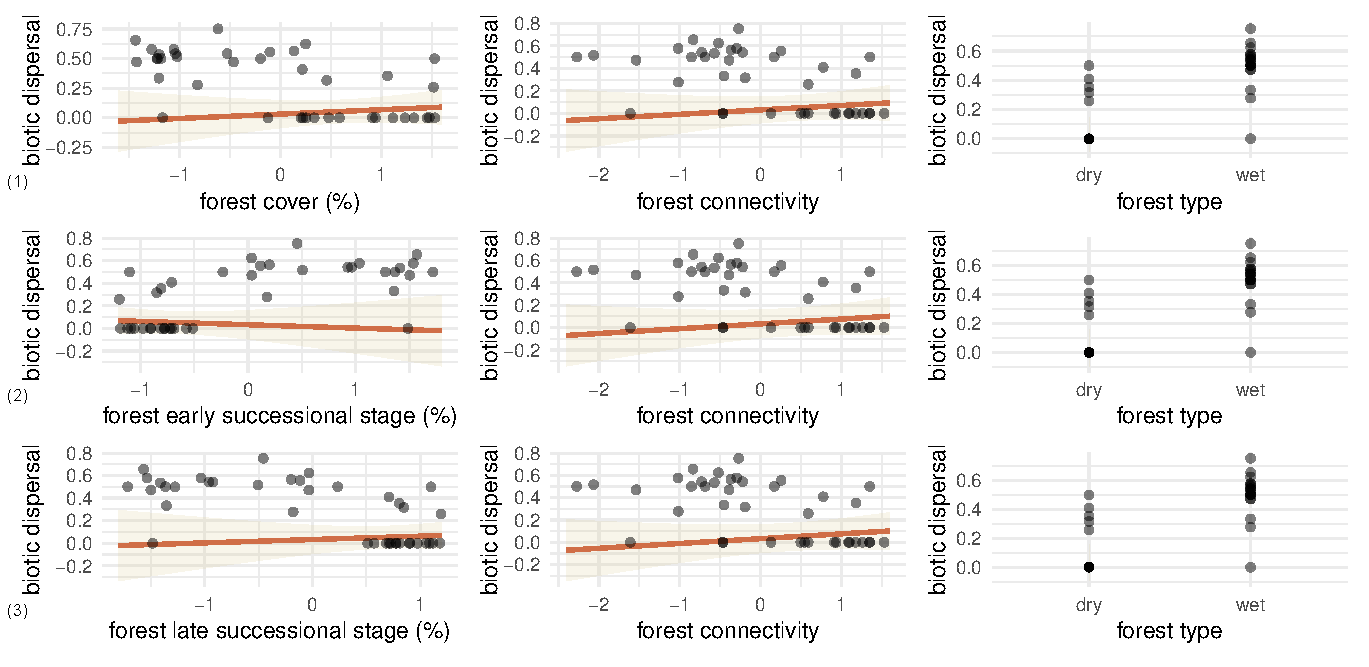
\includegraphics[width=0.95\linewidth,height=0.55\textheight,keepaspectratio]{Report/figures/models_biotic.pdf}%
}
\caption{\textit{Relationships between the proportion of biotically dispersed seeds of woody perennials and forest attributes. Each point represents the annual seed trap measurement per research plot. Linear regression lines (red) with 95\% confidence intervals (orange) show model predictions for models (1)-(3).}}
\label{fig:mod_biotic}
\end{figure}

% abiotic dispersal --------------------------------------------
\newpage
\begin{table}[H]
\centering
\scriptsize % smaller font
\caption{\textit{Linear regression results for the proportion of abiotically dispersed seeds. Models (1)–(3) test the effects of forest cover, successional stage, connectivity, and forest type (wet vs. dry) on the proportion of abiotically dispersed seeds of woody perennials. Standard errors are in parentheses.}}
\begin{tabularx}{\textwidth}{@{\extracolsep{3pt}}lXXX} 
\\[-1ex]\hline 
\hline \\[-1ex] 
 & \multicolumn{3}{c}{\textit{Dependent variable: Abiotic dispersal}} \\ 
\\[-1ex] & (1) & (2) & (3)\\ 
\hline \\[-0.8ex] 
Forest cover & $-$0.099 &  &  \\ 
 & (0.069) &  &  \\ 
Forest early successional stage &  & 0.055 &  \\ 
 &  & (0.078) &  \\ 
Forest late successional stage &  &  & $-$0.055 \\ 
 &  &  & (0.078) \\ 
Forest connectivity & 0.006 & $-$0.011 & $-$0.011 \\ 
 & (0.057) & (0.058) & (0.058) \\ 
Forest type (wet) & $-$0.473$^{***}$ & $-$0.429$^{***}$ & $-$0.429$^{***}$ \\ 
 & (0.133) & (0.151) & (0.151) \\ 
Constant & 0.814$^{***}$ & 0.792$^{***}$ & 0.792$^{***}$ \\ 
 & (0.075) & (0.083) & (0.083) \\ 
\hline \\[-0.8ex] 
Observations & 40 & 40 & 40 \\ 
R$^{2}$ & 0.408 & 0.383 & 0.383 \\ 
Adjusted R$^{2}$ & 0.359 & 0.331 & 0.331 \\ 
Residual Std. Error (df = 36) & 0.210 & 0.215 & 0.215 \\ 
F Statistic (df = 3; 36) & 8.282$^{***}$ & 7.435$^{***}$ & 7.435$^{***}$ \\ 
\hline 
\textit{Note:} & \multicolumn{3}{r}{$^{*}$p$<$0.1; $^{**}$p$<$0.05; $^{***}$p$<$0.01} \\ 
\end{tabularx} 
\label{tab:abiotic}
\end{table} 

\vspace{-2ex} % reduce space between table and figure

\begin{figure}[H]
\centering
\scriptsize % smaller caption font
\setlength{\fboxrule}{10pt}  % thinner frame
\setlength{\fboxsep}{0pt}    % no padding
\fcolorbox{framecol}{white}{%
  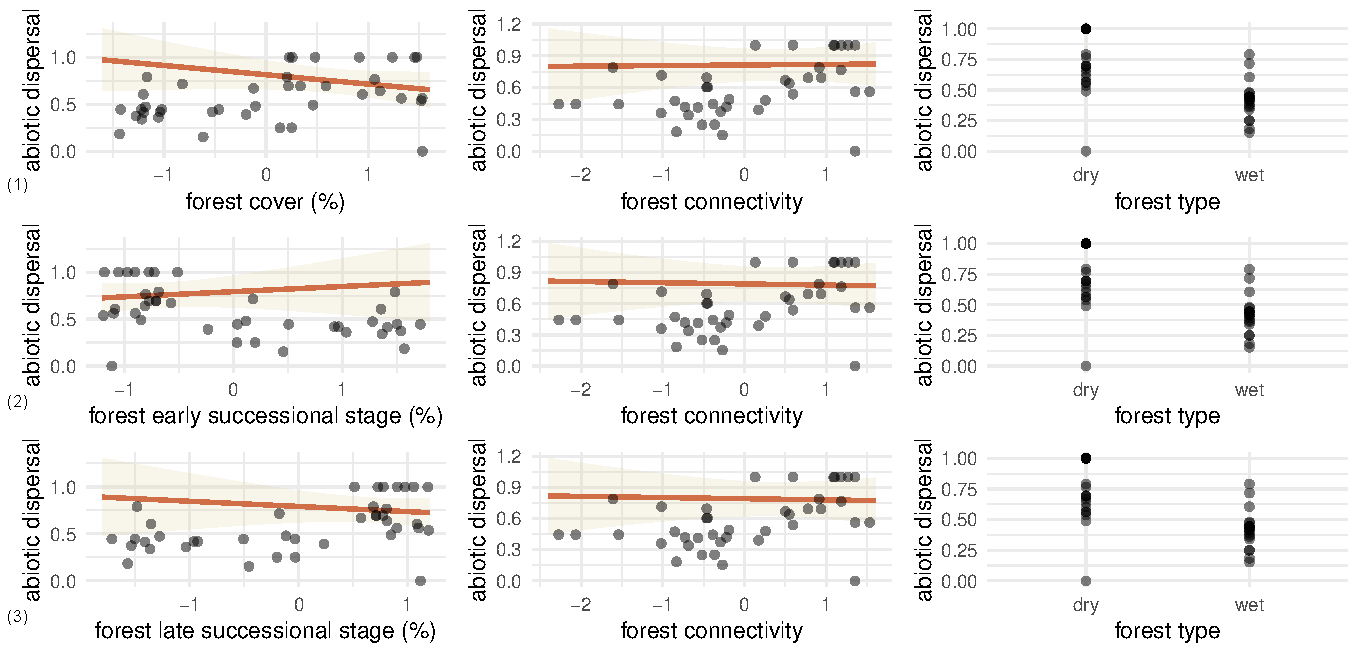
\includegraphics[width=0.95\linewidth,height=0.55\textheight,keepaspectratio]{Report/figures/models_abiotic.pdf}%
}
\caption{\textit{Relationships between the proportion of abiotically dispersed seeds of woody perennials and forest attributes. Each point represents the annual seed trap measurement per research plot. Linear regression lines (red) with 95\% confidence intervals (orange) show model predictions for models (1)-(3).}}
\label{fig:mod_abiotic}
\end{figure}


% generalist guild -----------------------------------------
\newpage
\begin{table}[H]
\centering
\scriptsize % smaller font
\caption{\textit{Linear regression results for the proportion of generalist guild seeds. Models (1)–(3) test the effects of forest cover, successional stage, connectivity, and forest type (wet vs. dry) on the proportion of generalist-dispersed seeds of woody perennials. Standard errors are in parentheses.}}
\begin{tabularx}{\textwidth}{@{\extracolsep{3pt}}lXXX} 
\\[-1ex]\hline 
\hline \\[-1ex] 
 & \multicolumn{3}{c}{\textit{Dependent variable: Generalist guild}} \\ 
\\[-1ex] & (1) & (2) & (3)\\ 
\hline \\[-0.8ex] 
Forest cover & $-$0.074$^{**}$ &  &  \\ 
 & (0.032) &  &  \\ 
Forest early successional stage &  & 0.030 &  \\ 
 &  & (0.038) &  \\ 
Forest late successional stage &  &  & $-$0.030 \\ 
 &  &  & (0.038) \\ 
Forest connectivity & $-$0.005 & $-$0.021 & $-$0.021 \\ 
 & (0.026) & (0.028) & (0.028) \\ 
Forest type (wet) & $-$0.071 & $-$0.023 & $-$0.023 \\ 
 & (0.062) & (0.072) & (0.072) \\ 
Constant & 0.221$^{***}$ & 0.197$^{***}$ & 0.197$^{***}$ \\ 
 & (0.034) & (0.040) & (0.040) \\ 
\hline \\[-0.8ex] 
Observations & 40 & 40 & 40 \\ 
R$^{2}$ & 0.231 & 0.130 & 0.130 \\ 
Adjusted R$^{2}$ & 0.167 & 0.057 & 0.057 \\ 
Residual Std. Error (df = 36) & 0.097 & 0.103 & 0.103 \\ 
F Statistic (df = 3; 36) & 3.599$^{**}$ & 1.792 & 1.792 \\ 
\hline 
\textit{Note:} & \multicolumn{3}{r}{$^{*}$p$<$0.1; $^{**}$p$<$0.05; $^{***}$p$<$0.01} \\ 
\end{tabularx} 
\label{tab:generalist}
\end{table} 

\vspace{-2ex} % reduce space between table and figure

\begin{figure}[H]
\centering
\scriptsize % smaller caption font
\setlength{\fboxrule}{10pt}  % thinner frame
\setlength{\fboxsep}{0pt}    % no padding
\fcolorbox{framecol}{white}{%
  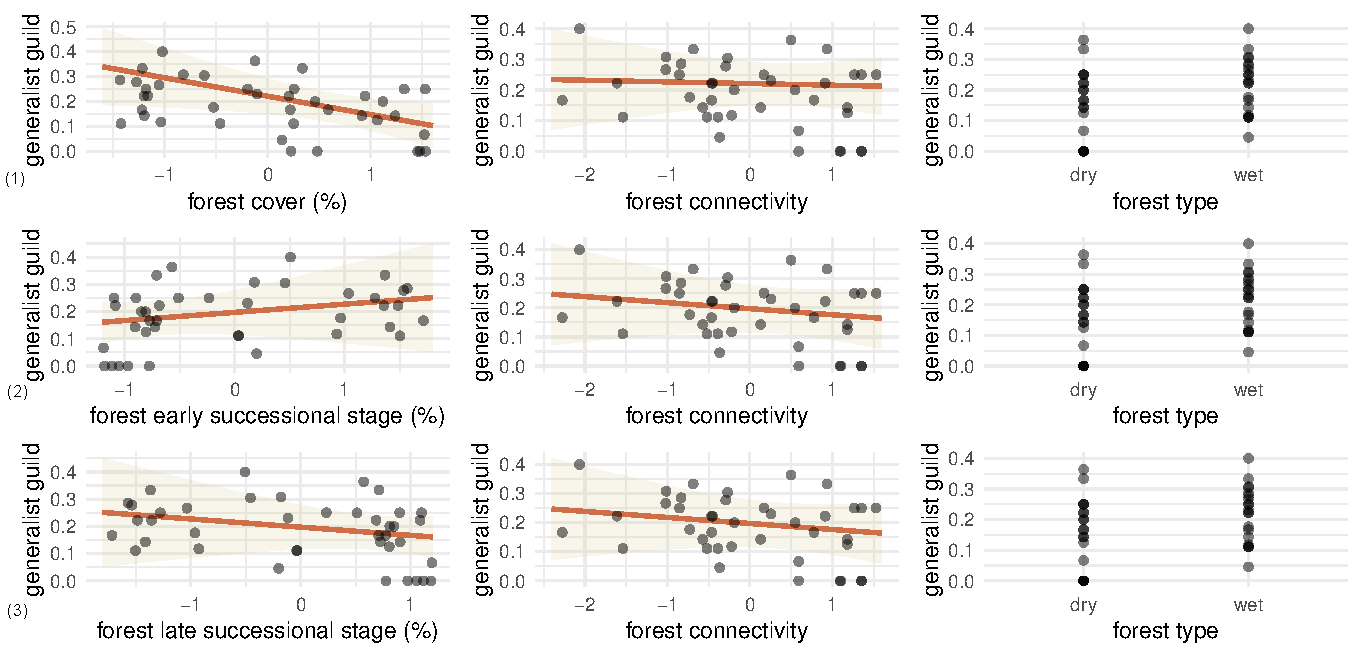
\includegraphics[width=0.95\linewidth,height=0.55\textheight,keepaspectratio]{Report/figures/models_generalist.pdf}%
}
\caption{\textit{Relationships between the proportion of generalist guild seeds of woody perennials and forest attributes. Each point represents the annual seed trap measurement per research plot. Linear regression lines (red) with 95\% confidence intervals (orange) show model predictions for models (1)-(3).}}
\label{fig:mod_generalist}
\end{figure}

% shadetolerant guild ----------------------------------------
\newpage
% \begin{table}[H]
% \centering
% \scriptsize % smaller font
% \caption{\textit{Linear regression results for the proportion of shade-tolerant guild seeds. Models (1)–(3) test the effects of forest cover, successional stage, connectivity, and forest type (wet vs. dry) on the proportion of shade-tolerant seeds of woody perennials. Standard errors are in parentheses.}}
% \begin{tabularx}{\textwidth}{@{\extracolsep{3pt}}lXXX} 
% \\[-1ex]\hline 
% \hline \\[-1ex] 
%  & \multicolumn{3}{c}{\textit{Dependent variable: Shadetolerant guild}} \\ 
% \\[-1ex] & (1) & (2) & (3)\\ 
% \hline \\[-0.8ex] 
% Forest cover & 0.232 &  &  \\ 
%  & (0.189) &  &  \\ 
% Forest early successional stage &  & $-$0.165 &  \\ 
%  &  & (0.211) &  \\ 
% Forest late successional stage &  &  & 0.165 \\ 
%  &  &  & (0.211) \\ 
% Forest connectivity & $-$0.024 & 0.009 & 0.009 \\ 
%  & (0.157) & (0.157) & (0.157) \\ 
% Forest type (wet) & 0.501 & 0.448 & 0.448 \\ 
%  & (0.366) & (0.406) & (0.406) \\ 
% Constant & $-$0.590$^{***}$ & $-$0.562$^{**}$ & $-$0.562$^{**}$ \\ 
%  & (0.206) & (0.224) & (0.224) \\ 
% \hline \\[-0.8ex] 
% Observations & 40 & 40 & 40 \\ 
% R$^{2}$ & 0.055 & 0.035 & 0.035 \\ 
% Log Likelihood & 22.208 & 21.774 & 21.774 \\ 
% \hline 
% \textit{Note:} & \multicolumn{3}{r}{$^{*}$p$<$0.1; $^{**}$p$<$0.05; $^{***}$p$<$0.01} \\ 
% \end{tabularx} 
% \label{tab:shadetolerant}
% \end{table} 

\begin{table}[H]
\centering
\scriptsize
\caption{\textit{Gamlss BEZI model results for the proportion of shade-tolerant guild seeds. Models (1)–(3) test the effects of forest cover, successional stage, connectivity, and forest type (wet vs. dry) on the proportion of shade-tolerant seeds of woody perennials. Standard errors are in parentheses.}}
\begin{tabularx}{\textwidth}{@{\extracolsep{3pt}}lXXX} 
\\[-1ex]\hline 
\hline \\[-1ex] 
 & \multicolumn{3}{c}{\textit{Dependent variable: Shadetolerant guild}} \\ 
\\[-1ex] & (1) & (2) & (3)\\ 
\hline \\[-0.8ex] 
Forest cover & 0.038 &  &  \\ 
 & (0.189) &  &  \\ 
Forest early successional stage &  & $-$0.130 &  \\ 
 &  & (0.219) &  \\ 
Forest late successional stage &  &  & 0.130 \\ 
 &  &  & (0.219) \\ 
Forest connectivity & 0.132 & 0.125 & 0.125 \\ 
 & (0.156) & (0.149) & (0.149) \\ 
Forest type (wet) & 0.024 & 0.180 & 0.180 \\ 
 & (0.378) & (0.440) & (0.440) \\ 
Constant (Intercept, Mu) & $-$1.840$^{***}$ & $-$1.921$^{***}$ & $-$1.921$^{***}$ \\ 
 & (0.226) & (0.253) & (0.253) \\ 
\hline \\[-0.8ex] 
Sigma (dispersion) & 3.569$^{***}$ & 3.582$^{***}$ & 3.582$^{***}$ \\
 & (0.277) & (0.277) & (0.277) \\
Nu (zero-inflation) Intercept & $-$0.619$^{.}$ & $-$0.619$^{.}$ & $-$0.619$^{.}$ \\
 & (0.332) & (0.332) & (0.332) \\
Observations & 40 & 40 & 40 \\ 
Global Deviance & -25.993 & -26.300 & -26.300 \\ 
AIC & -13.993 & -14.300 & -14.300 \\ 
SBC & -3.860 & -4.167 & -4.167 \\ 
\hline 
\textit{Note:} & \multicolumn{3}{r}{$^{.}$p$<$0.1; $^{*}$p$<$0.05; $^{**}$p$<$0.01; $^{***}$p$<$0.001} \\ 
\end{tabularx} 
\label{tab:shadetolerant_gamlss}
\end{table}

\vspace{-2ex} % reduce space between table and figure

% \begin{figure}[H]
% \centering
% \scriptsize % smaller caption font
% \setlength{\fboxrule}{10pt}  % thinner frame
% \setlength{\fboxsep}{0pt}    % no padding
% \fcolorbox{framecol}{white}{%
%   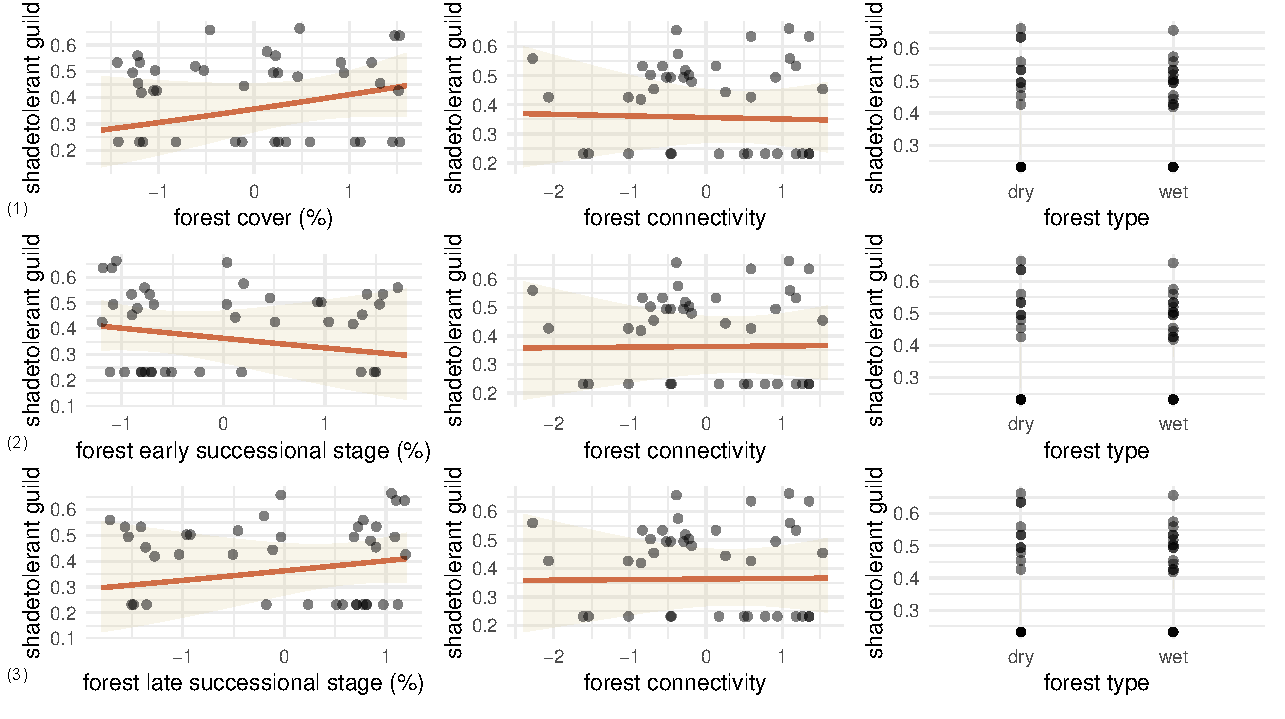
\includegraphics[width=0.95\linewidth,height=0.55\textheight,keepaspectratio]{Report/figures/models_shadetolerant.pdf}%
% }
% \caption{\textit{Relationships between the proportion of shade-tolerant guild seeds of woody perennials and forest attributes. Each point represents the annual seed trap measurement per research plot. Linear regression lines (red) with 95\% confidence intervals (orange) show model predictions for models (1)-(3).}}
% \label{fig:mod_shadetolerant}
% \end{figure}



% pioneer guild --------------------------------------------
\newpage
\begin{table}[H]
\centering
\scriptsize % smaller font
\caption{\textit{Linear regression results for the proportion of pioneer guild seeds. Models (1)–(3) test the effects of forest cover, successional stage, connectivity, and forest type (wet vs. dry) on the proportion of pioneer-dispersed seeds of woody perennials. Standard errors are in parentheses.}}
\begin{tabularx}{\textwidth}{@{\extracolsep{3pt}}lXXX} 
\\[-1ex]\hline 
\hline \\[-1ex] 
 & \multicolumn{3}{c}{\textit{Dependent variable: Pioneer guild}} \\ 
\\[-1ex] & (1) & (2) & (3)\\ 
\hline \\[-0.8ex] 
Forest cover & 0.004 &  &  \\ 
 & (0.034) &  &  \\ 
Forest early successional stage &  & $-$0.022 &  \\ 
 &  & (0.038) &  \\ 
Forest late successional stage &  &  & 0.022 \\ 
 &  &  & (0.038) \\ 
Forest connectivity & $-$0.019 & $-$0.023 & $-$0.023 \\ 
 & (0.029) & (0.028) & (0.028) \\ 
Forest type (wet) & 0.042 & 0.067 & 0.067 \\ 
 & (0.066) & (0.073) & (0.073) \\ 
Constant & 0.399$^{***}$ & 0.386$^{***}$ & 0.386$^{***}$ \\ 
 & (0.037) & (0.040) & (0.040) \\ 
\hline \\[-0.8ex] 
Observations & 40 & 40 & 40 \\ 
R$^{2}$ & 0.102 & 0.110 & 0.110 \\ 
Adjusted R$^{2}$ & 0.027 & 0.036 & 0.036 \\ 
Residual Std. Error (df = 36) & 0.105 & 0.104 & 0.104 \\ 
F Statistic (df = 3; 36) & 1.361 & 1.484 & 1.484 \\ 
\hline 
\textit{Note:} & \multicolumn{3}{r}{$^{*}$p$<$0.1; $^{**}$p$<$0.05; $^{***}$p$<$0.01} \\ 
\end{tabularx} 
\label{tab:pioneer}
\end{table} 

\vspace{-2ex} % reduce space between table and figure

\begin{figure}[H]
\centering
\scriptsize % smaller caption font
\setlength{\fboxrule}{10pt}  % thinner frame
\setlength{\fboxsep}{0pt}    % no padding
\fcolorbox{framecol}{white}{%
  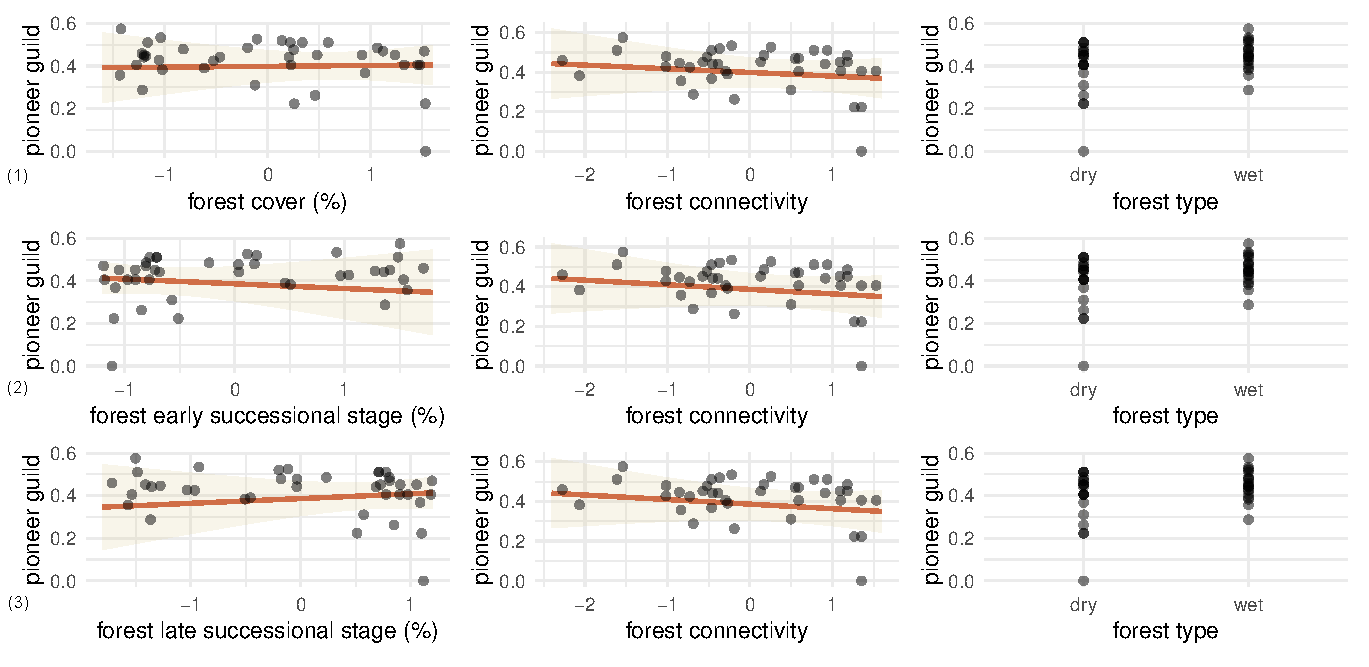
\includegraphics[width=0.95\linewidth,height=0.55\textheight,keepaspectratio]{Report/figures/models_pioneer.pdf}%
}
\caption{\textit{Relationships between the proportion of pioneer guild seeds of woody perennials and forest attributes. Each point represents the annual seed trap measurement per research plot. Linear regression lines (red) with 95\% confidence intervals (orange) show model predictions for models (1)-(3).}}
\label{fig:mod_pioneer}
\end{figure}

\newpage
\section{Table of content of the zip file that accompanies the thesis report}
\begin{itemize}
    \item Documentation
    \item Report
    \item Midterm \& Final presentation (pptx)
    \item Datasets (used and created)
    \item Visuals (figures \& maps)
    \item Scripts
\end{itemize}
